\documentclass[a4paper, 12pt]{article}
\usepackage[margin=2.5cm]{geometry}
\usepackage[swedish]{babel}
\usepackage[T1]{fontenc}
\usepackage[utf8]{inputenc}
\usepackage{mathtools}
\usepackage{graphicx}
\usepackage{hyperref}
\usepackage{url}
\usepackage{array}
\usepackage[dvipsnames]{xcolor}
\usepackage{csquotes}
\usepackage{cite}
\usepackage{tikz}
\usepackage{subcaption}

\begin{document}

\begin{titlepage}
    % Uppsala logotyp
    \begin{tikzpicture}[remember picture, overlay]
        \node [anchor=north west, inner sep=30pt]  at (current page.north west)
            {
\includegraphics[height=4cm]{logo_uu_se.png}};
    \end{tikzpicture}

    \begin{center}
        % Rubrik
        {\LARGE \textbf{Nationskompassen} \\ \large Pubrundor för studenter i Uppsala} \\[2cm]

        % Nationskompassen logotyp
        \includegraphics[height=10cm]{logo_nationskompassen_utantext.png} \\[1cm]

        % Författare och handledare
        \textbf{Projektgrupp 50} \\
        Anton Äng \\
        Alexander Brundin \\
        Emil Reimegård \\[0.5cm]
        Handledare: Matilda Blomqvist \\

        % Datum
        \today

        % Kursinfomration
        \vfill
        Projektrapport för kursen Programkonstruktion och datastrukturer \\
        Uppsala Universitet \\
        VT 26
    \end{center}
\end{titlepage}

\newpage

\tableofcontents

\newpage
% Introduktion
\section{Introduktion}
    Uppsala som studentstad präglas av dess nationer och de aktiviteter som med nationerna kommer till. Nationsguiden är en webbplats som samlar in och tillhandahåller information om de olika nationerna i Uppsala, inklusive deras evenemang, öppettider och kontaktinformation. Denna webbplats är avsedd att hjälpa både nya och befintliga studenter att navigera i det rika utbuted av nationer i Uppsala. Detta arbete menar dock att webplatsen saknar viss funktionallitet. Möjligheten att kombinera nationers aktiviteter och evenemang är något som Nationsguiden inte själva implementerat, det initiativet står istället användaren för och kan vara tidskrävande. Nationskompassen som program ses kunna komplettera denna brist i funktionallitet hos Nationsguiden, ihop om att öka användarvänligheten för studenter på Uppsala Universitet.


    Nationskompassen är ett program som utnyttjar den information som Nationsguiden tillhandahåller för att skapa den kortaste pubrundan möjlig utfirån de nationspubar som för ett givet datum är öppna, vart användaren vill påbörja sin pubrunda samt hur många nationspubbar som rundan ska innehålla. Genom detta erbjuder Nationskompassen en effektiv lösning på att slå samman nationser evenemang och planera pubrundor.

% Guide
\section{Guide till Nationskompassen}

% Dokumentation
\section{Programdokumentation}

    \subsection{Allmän design på programmet}
        Nationskompassen är en pubrundsplanerare för Uppsalas studentnationer. Den låter användaren välja startpub och längden på rutten Därefter hämtar den data från hemsidan nationsguiden.se och genererar den geografiskt sett kortaste pubrundan baserat på användarens val. Programmet Nationskompassen är uppdelat i sex moduler med olika ansvarsområden:
        \begin{itemize}
            \item \textbf{\texttt{collect\_data}} - Hämtar information från nationsguiden.se
            \item \textbf{\texttt{extract\_essential\_data}} - Extraherar relevant information från collect\_data
            \item \textbf{\texttt{build\_nationgraph}} - Använder relevant information för att konstruera en viktad graf
            \item \textbf{\texttt{create\_route}} - Skapar en pubrunda utifrån en viktad graf
            \item \textbf{\texttt{user\_input}} - Möjliggör för användaren att interagera med programet
            \item \textbf{\texttt{main}} - Den drivande modulen som kordinerar de andra modulerna
        \end{itemize}
        Strukturen i programmet är sekventiell. MainGraph anropar CollectDataGraph som hämtar rådatan. Den datan skickar MainGraph vidare till HandleDataGraph som bearbetar och beräknar den pubrunda som har kortast avstånd. Slutligen skriver MainGraph ut den genererade pubrundan till konsolen så att användaren kan se den.

    \subsection{Viktiga datastrukturer och algoritmer}

        \subsubsection{Datastrukturer}

            \paragraph{NationNode}
                är den centrala datastrukturen i programmet. Varje nationspub representeras som en NationNode. Den innehåller organisationsnamn, pubnamn, öppetider, kontaktinformation, geografiska koordinater samt nationens vikt som används vid avståndsberäkningar.

            \paragraph{NationMatrix}
                är en tvådimensionell array av NationNodes som fungerar som en viktad matris. Raden $i$ och kolumnen $j$ håller en kopia av NationNode$(j)$ där vikten är satt till avståndet mellan nation$(i)$ och nation$(j)$. Diagonalelementen, det vill säga en nations avstånd till sig själv, är alltid 0.

            \paragraph{NationIndex}
                är en Map av typ \texttt{\{string, number\}} som kopplar nationsnamnet till ett index $(i)$ i NationMatrix för att snabbt kunna slå upp ett nationsindex.

            \paragraph{Set$\langle$number$\rangle$}
                är ett set som håller redan besökta nationer för att säkerställa att samma nation inte besöks två gånger.
            
            \paragraph{Pair$\langle$string, number$\rangle$}
                används för att ta emot användarens val: startpub och antal nationer.

        \subsubsection{Algoritmer}
            Programmet använder två viktiga algoritmer som återfinns i \texttt{get\_distance} och \texttt{nearest\_nation}. \texttt{get\_distance} utnyttjar Pythagoras sats för att beräkna avståndet mellan två nationer med hjälp av deras latitud- och longitudkoordinater. \texttt{nearest\_nation} är en så kallad girig närmaste-granne-algoritm. Det innebär att den vid varje nytt steg under sökningen gör valet enbart baserat på vad som är bäst i stunden. I \texttt{nearest\_nation} innebär det att den alltid väljer den nation som ligger närmast den nation den befinner sig på just nu.

    \subsection{Moduler och bibliotek}
        Nationskompassen importerar fyra bibliotek: \texttt{nation}, \texttt{list}, \texttt{hashtables} och \texttt{graphs}. Från \texttt{list}-biblioteket hämtas typen \texttt{Pair} och konstruktorfunktionen \texttt{pair}, som används för att representera användarens val som ett par av startnation och antal stopp. \texttt{nation}-biblioteket innehåller alla relevanta typer för programmet, beskrivna i avsnitt 3.2, samt en statisk array som håller koordinaterna till alla nationer.

    \subsection{Viktiga funktioner}
        \begin{itemize}
            \item \texttt{main()} är startpunkten för hela programmet. Anropar relevanta funktioner för datainsamling och bearbetning samt hanterar eventuella fel med try/catch.
            \item \texttt{getEvents()} skickar ett anrop till nationsguiden.se och returnerar en array av typen \texttt{NationGuideCategory}.
            \item \texttt{get\_open\_pubs(json\_parsed)} filtrerar en array av typen \texttt{Array\textless{}NationGuideCategory\textgreater{}} baserat på event som tillhör kategorin ''pub'' och returnerar en array med \texttt{NationGuideEvent}.
            \item \texttt{extract\_essentials()} omvandlar en array av typen \texttt{Array\textless{}NationGuideEvent\textgreater{}} till en array av \texttt{NationNode} genom att extrahera relevant information från varje instans av \texttt{NationGuideEvent}. Använder hjälpfunktionen \texttt{get\_organiser\_coordinates()} för att hämta nationens koordinater från koordinatarrayen i nationsbiblioteket. Returnerar en array av \texttt{NationNode}.
            \item \texttt{build\_nation\_distance\_matrix()} bygger en viktad tvådimensionell matris av typen \texttt{NationMatrix} baserat på en array av \texttt{NationNode}. Bestämmer vikten med hjälp av \texttt{get\_distance()} som beräknar avståndet mellan två nationer med hjälp av Pythagoras sats.
            \item \texttt{build\_nation\_index()} kopplar varje nationnamn till ett index med den inbyggda Map-funktionen. Används för att snabbt slå upp ett nationsindex.
            \item \texttt{nearest\_nation()} hittar den närmaste, ej besökta nationen som inte är den nuvarande. Returnerar den närmast tillgängliga nationen.
            \item \texttt{create\_route()} tar emot användarens val av startnation samt antal pubar som önskas besökas. Skapar pubrundan med hjälp av repetitiva anrop till \texttt{nearest\_nation()} tills pubrundan uppfyller användarens krav eller tills det inte finns fler pubar att besöka.
        \end{itemize}

    \subsection{Kontrollflöde och hjälpfunktioner}

        Programmet börjar i \texttt{main()}, som koordinerar samtliga anrop under programmets körning. Det första steget är att hämta data, vilket sker genom ett anrop till \texttt{getEvents()}. Den funktionen skickar gör anrop till nationsguiden.se och returnerar rådatan som en array av \texttt{NationGuideCategory}.


        Rådatan skickas vidare till \texttt{get\_open\_pubs()}, som filtrerar bort alla evenemang som inte tillhör kategorin ''pub'' och returnerar en renare array av \texttt{NationGuideEvent}. Denna array skickas i sin tur till \texttt{extract\_essentials()}, som omvandlar varje event till en \texttt{NationNode}. För att göra det anropar \texttt{extract\_essentials()} sin privata hjälpfunktion \texttt{get\_organiser\_coordinates()}, vilken slår upp nationens GPS-koordinater i den statiska koordinatarrayen från nationsbiblioteket. Koordinaterna läggs sedan in i \texttt{NationNode}-objektet.


        Den resulterande arrayen av \texttt{NationNode} skickas slutligen till \texttt{create\_route()} tillsammans med användarens val av startnation och antal stopp. Inuti \texttt{create\_route()} sker en intern kedja av anrop: först byggs distansmatrisen upp via \texttt{build\_nation\_distance\_matrix()}, som internt anropar sin hjälpfunktion \texttt{get\_distance()} för att beräknar avståndet mellan varje nationpar. Därefter anropas \texttt{build\_nation\_index()} för att kunna slå upp startnationers index i matrisen. Sedan itererar \texttt{create\_route()} och anropar \texttt{nearest\_nation()} upprepade gånger tills pubrundan uppfyller det antal stopp som användaren angett.


        Hjälpfunktionerna \texttt{get\_organiser\_coordinates()} och \texttt{get\_distance()} är båda privata, det vill säga de är definierade inuti sina respektive föräldrafunktioner och anropas aldrig direkt utifrån. De används enbart för att hålla föräldrafunktionernas logik läsbar och välstrukturerad.


        Slutligen returnerar \texttt{create\_route()} den färdiga pubrundan som en array av strängar, vilken \texttt{main()} skriver ut till konsolen.


\section{Testning}
    Testning är en central del av mjukvareutveckling som syftar till att säkerställa en programvaras pålitlighet, funktionalitet och kvalitet. Som en del av detta projektarbete och utvecklingen av Nationskompassen användes testning för att verifiera att de olika komponenterna i programmet fungerar och samverkar som tänkt. Eftersom den data som tillhandahåls av nationsguiden.se kan variera, är det avgörande att programet kan hantera dessa variationer korrekt. Testningen utfördes på två nivåer: enhetstestning och integrationstestning. Enhetstestning fokuserade på att testa individuella funktioner och moduler i isolering, medan integrationstestningen syftade till att säkerställa huruvida data flödar genom programets olika komponenter som tänkt. Testningen utfördest med Jest (ref här och förklaring). All testning genomfördes med syntetisk data och är uppdelad i tre delar, en för varje modul av programmet. (skriv också --coverage grejer)

    \subsection{\texttt{extract\_essential\_data}}
        Här testades funktionerna \texttt{get\_open\_pubs()} och \texttt{extract\_essentials()}. Testerna täcker olika scenarion, inklusive fall där det inte finns några öppna pubar, fall där det finns flera öppna pubar och fall där datan innehåller oväntade format eller saknade fält. Testerna verifierar att \texttt{get\_open\_pubs()} korrekt filtrerar ut endast de evenemang som tillhör kategorin 'Pub' och att \texttt{extract\_essentials()} korrekt extraherar och omvandlar informationen till \texttt{NationNode}-objekt. Därefter utfördes även tester på särskilda/få förekommande scenarion, såsom de fall där datan innehåller oväntade format eller där viss data förekommer i dubbletter. Samtliga testningar för Nationskompassen följer liknande struktur, därav agerar \hyperref[fig:overview_tests]{Fig.1} exempel för en överblick på en moduls tester och \hyperref[fig:example_tests]{Fig.2} exempel för hur ett tester kan se ut.

    \subsection{\texttt{build\_nationGraph}}
        I denna del av testningen säkerställndes att steget mellan skapandet av en \texttt{NationNode} till en \texttt{NationMatrix} var korrek genom funktionerna \texttt{get\_distance()}, \texttt{build\_nation\_index()} samt \texttt{build\_nation\_distance\_matrix()}. Testerna säkerställer bland annat att \texttt{get\_distance()} korrekt beräknar avstånd mellan två \texttt{NationNode}, att \texttt{build\_nation\_index()} korrekt tillger en \texttt{NationNode} ett index och att \texttt{build\_nation\_distance\_matrix()} returnerar en pålitlig struktur av en \texttt{NationMatrix}. Därefter säkerställdes även att funktionerna fungerade som tänkt i ett integrationstest, där en \texttt{NationMatrix} skapades och vardera \texttt{NationNode} tilldelades ett giltigt index.

    \subsection{\texttt{create\_route}}
        I sista steget av testningen säkerställdes att skapandet av pubrundan var pålitlig genom funktionerna \texttt{nearest\_nation()} samt \texttt{create\_route()}. Testerna verifierade exempelvis att en pubrunda inte innehöll dubbletter av nationer och att pubrundans längd var anpassad både efter efterfrågan men också antalet tillgängliga nationspubbar.

\section{Diskusion}
    \subsection{Val under projektets gång}
        Projeket inleddes med en vision där användaren skulle använda programmet i ett grafiskt användargränssnitt. Flera olika tekniker diskuterades innan det fastställdes att HTML skulle användas för att representera datan grafiskt. Denna vision ändrades dock tidigt under projektets gång och istället för ett grafiskt användargränssnitt så exekveras programmet direkt i terminalen. Anledningen till detta var främst tidsbrist, men även att den grafiska delen inte var en del av kursens lärandemål.


        Ett annat val som gjordes tidigt in i projektet var hurvida datan som skulle användas var riktig data eller om den skulle ha varit syntetisk data. Det beslutades om att använda riktig data som hämtades från Nationsguiden, detta för att det skulle vara mer realistiskt och för att det skulle vara mer intressant att arbeta med riktig data. Detta ledde fram till nästa problem, hur skulle datan hämtas? 


        Där togs beslutet att huvudfokuset med projektet är inte att implementera en form of web scraper, utan mer att hantera den inhämtade datan. Därför valdes att använda en AI-assistet för att generera funktionen som hämtar datan från nationsguiden.se och parsar den till ett format som enklare kan hanteras.

        
        Det sista stora beslutet som togs var att övergå från den ursprungliga visionen av att programmet skulle spara datan för varje nation i hashtabeller, till att istället representera nationerna som noder i en viktad graf. För att sedan med hjälp av en grafalgoritm hitta den kortaste vägen mellan norderna. Detta beslut togs eftersom relationerna mellan nationerna bättre kan beskrivas som ett nätverk. En graf gör det möjligt att representera nationerna som noder och avstånden mellan dem som vikter på kanterna. 

    \subsection{svagheter}
        Programmets främsta svaghet finns redan innan inhämtningen av datan, för att hämta datan så måste funktionen uppdateras med en nonce värde, en sträng med nummer som uppdateras 2 gånger under dagen som hämtas från nationsguiden.se. 

    \subsection{Framtida projekt}
        Hade det funnits mer tid så hade det varit intreesant att få implemetera det grafiska användargränssnittet som nämndes under. Det hade bidragit till användaupplevelsen och gjort det mer tillgängligt för användare som inte är bekväma med att använda terminalen.


        Det hade också varit bra att hitta en metod så nonce värdet inte behöver uppdateras manuellt varje gång datan ska hämtas. Det diskuterades olika ideer för att lösa detta. Bland annat genom att använda TypeScript kompatibla playwright, som hade kunnat användas för att spela in stegen som behövs för att hämta nonce värdet. För att därefter köra den delen av programmet innan datan hämtas.


        \small (fler valmöjligheter, en slutdestination, mer information om evenemang, möjlighet att spara sina rutter - inloggning eller .txt eller .pdf - grafiskt gränssnitt, mobilanpassning, förslag på slutdestinationer utifrån klubbar, etc.)

\section{Sammanfattning, kan slås ihop med diskussionen, eller subsection}

\newpage
\appendix
\section*{Bilagor}
\addcontentsline{toc}{section}{Bilagor}

\begin{figure}[htbp]
    \centering

        \begin{subfigure}{0.6\textwidth}
            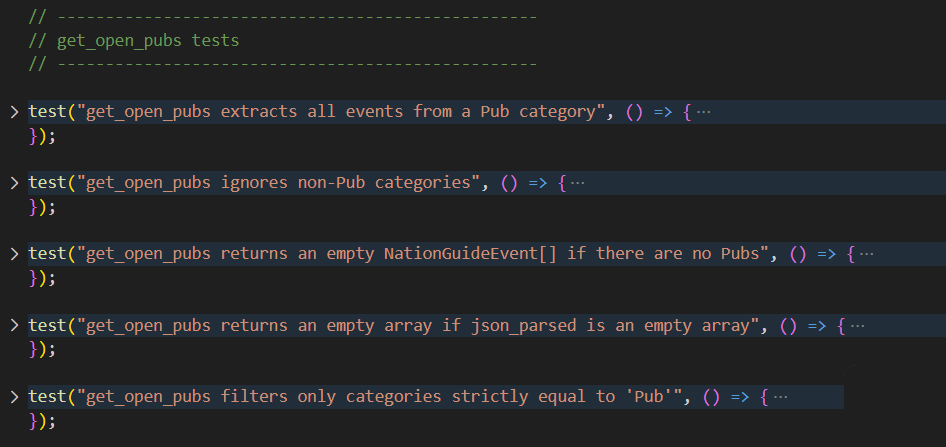
\includegraphics[width=\linewidth]{./jest_bilder/get_open_pubs.test.png}
            \caption{Tester för \texttt{get\_open\_pubs()}}
        \end{subfigure}

        \begin{subfigure}{0.6\textwidth}
            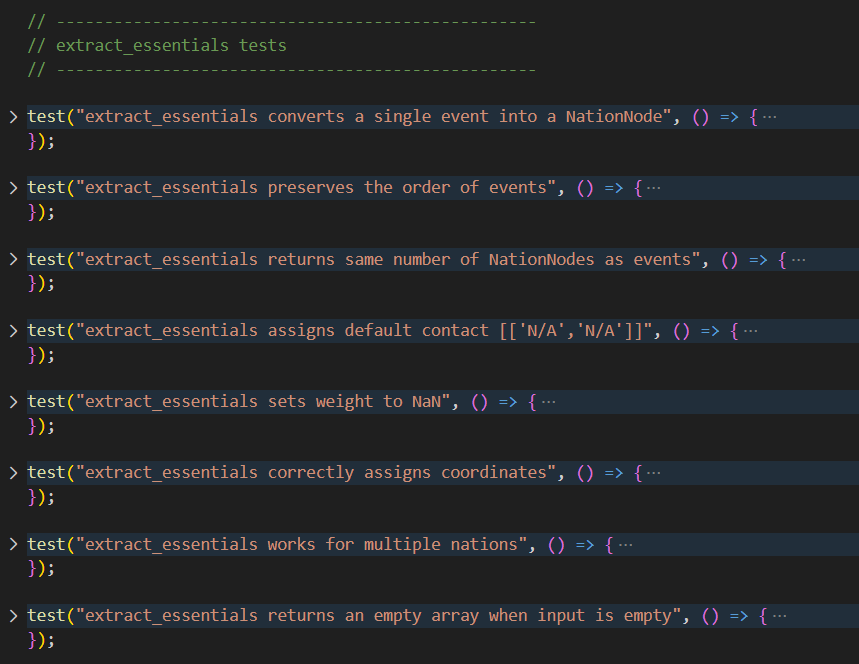
\includegraphics[width=\linewidth]{./jest_bilder/extract_essentials.test.png}
            \caption{Tester för \texttt{extract\_essentials()}}
        \end{subfigure}

        \begin{subfigure}{0.6\textwidth}
            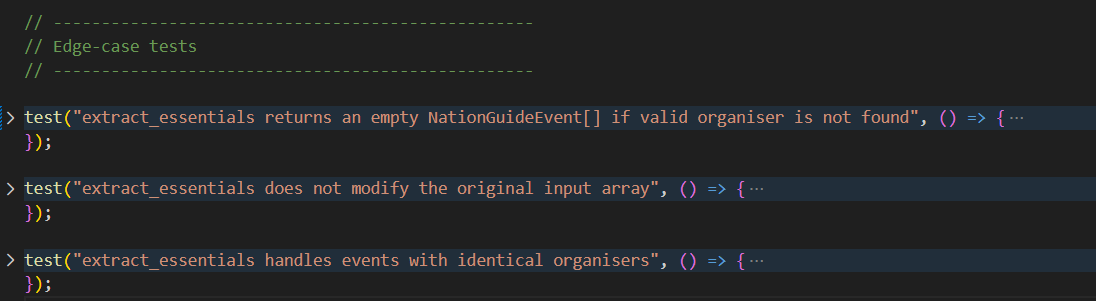
\includegraphics[width=\linewidth]{./jest_bilder/extract_essential_data_edge.test.png}
            \caption{Edge-case tester}
        \end{subfigure}

        \caption{Översikt av Jest-tester för modulen \texttt{extract\_essential\_data}.}
        \phantomsection
        \label{fig:overview_tests}
\end{figure}
\newpage
\begin{figure}[htbp]
    \centering

        \begin{subfigure}{0.7\textwidth}
            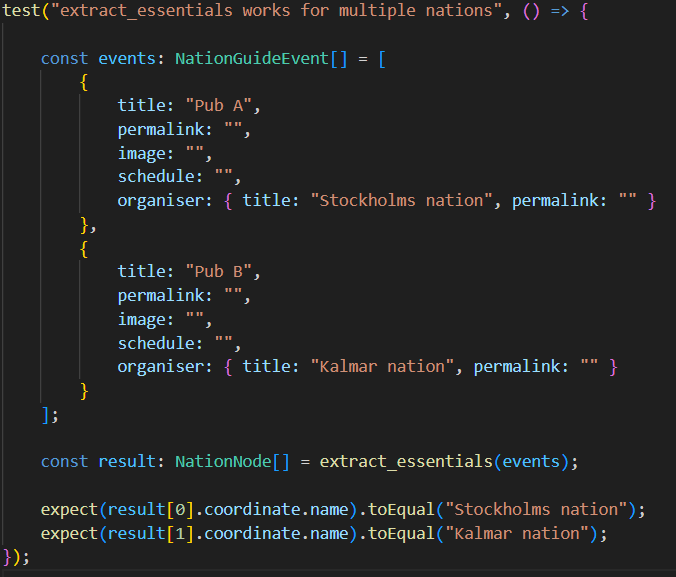
\includegraphics[width=\linewidth]{./jest_bilder/ex_test.png}
            \caption{Exempel på standardtest}
        \end{subfigure}

        \hfill

        \begin{subfigure}{0.7\textwidth}
            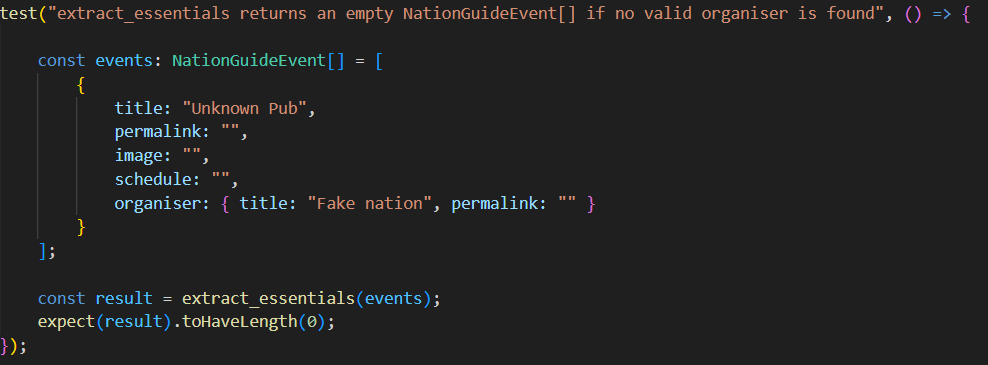
\includegraphics[width=\linewidth]{./jest_bilder/ex_test_edge.png}
            \caption{Exempel på edge-case test}
        \end{subfigure}
        
        \caption{Exempel på individuella Jest-tester för extraktionsfunktionerna.}
        \phantomsection
        \label{fig:example_tests}
\end{figure}

\end{document}